\titleformat{\chapter}[display]{\normalfont\LARGE\bfseries}{}{1em}{\thechapter.~}

\chapter{Laboratorio: Lógica convencional, Arranque-pare sencillo y reversible.}


\section{Objetivos}
Este  laboratorio busca:
\begin{itemize}
	{\small
	 \item  Estudiar  las representaciones simbólicas normalizadas de los elementos de control eléctrico, según norma NEMA ICS 19-2002 y IEC 60617.
	 \item Seleccionar contactores y relevadores térmicos.
	 \item  Estudiar la representación gráfica del estandar NEMA ICS 19-2002 o IEC 60617. 
	 \item  Diseñar e implementar circuitos de control para arranque sencillo de un motor trifásico.
	 \item  Diseñar e implementar circuitos de control para arranque-pare reversible de un  motor trifásico.
 }
\end{itemize} 

 
\section{Equipos y materiales}
Para este laboratorio de necesitaran:
\begin{itemize}
	{\small \item 1 motor trifásico 1/2 hp de 3 puntas
	\item 1 relevador térmico
	\item 1 botón pulsar cerrado
	\item 2 botones pulsadores abiertos
	\item 1 multimetro.
}
\end{itemize}

\section{Marco de referencia}

El control eléctrico de motores es un conjunto de técnicas y dispositivos utilizados para administrar la operación de un motor eléctrico. El control eléctrico de motores se utiliza, para regular la velocidad, el par, la dirección de rotación, el arranque y el frenado del motor.

En general, el control eléctrico de motores implica la utilización de circuitos electrónicos y sistemas de control para ajustar el suministro de energía eléctrica al motor y así lograr la operación deseada. El control eléctrico de motores se aplica en una amplia gama de aplicaciones, desde equipos de producción industrial hasta electrodomésticos y sistemas de transporte.

\subsection{Contactor y relevador térmico}

Un contactor es un dispositivo electromecánico utilizado para controlar la conexión y desconexión de motores eléctricos u otros equipos eléctricos de alta potencia como; calentadores eléctricos, luminarias, banco de capacitores, etc. Los contactores consisten en un electroimán que activa los contactos eléctricos para permitir o interrumpir el flujo de corriente eléctrica hacia el motor, un ejemplo de un contactor de uso general se muestra en la Figura \ref{fig:contactor}. Los contactores suelen utilizarse en combinación con los relés de sobrecarga.


\begin{figure}
	\centering
	\begin{subfigure}[b]{0.4\textwidth}
		\centering
		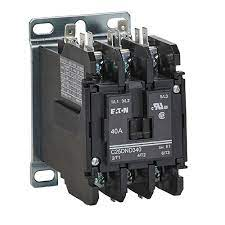
\includegraphics[width=\textwidth]{Imagenes/Contactor}
		\caption{Contactor de proposito general Eaton \cite{Eaton1}.}
		\label{fig:contactor}
	\end{subfigure}
\hfill
	\begin{subfigure}[b]{0.4\textwidth}
		\centering
		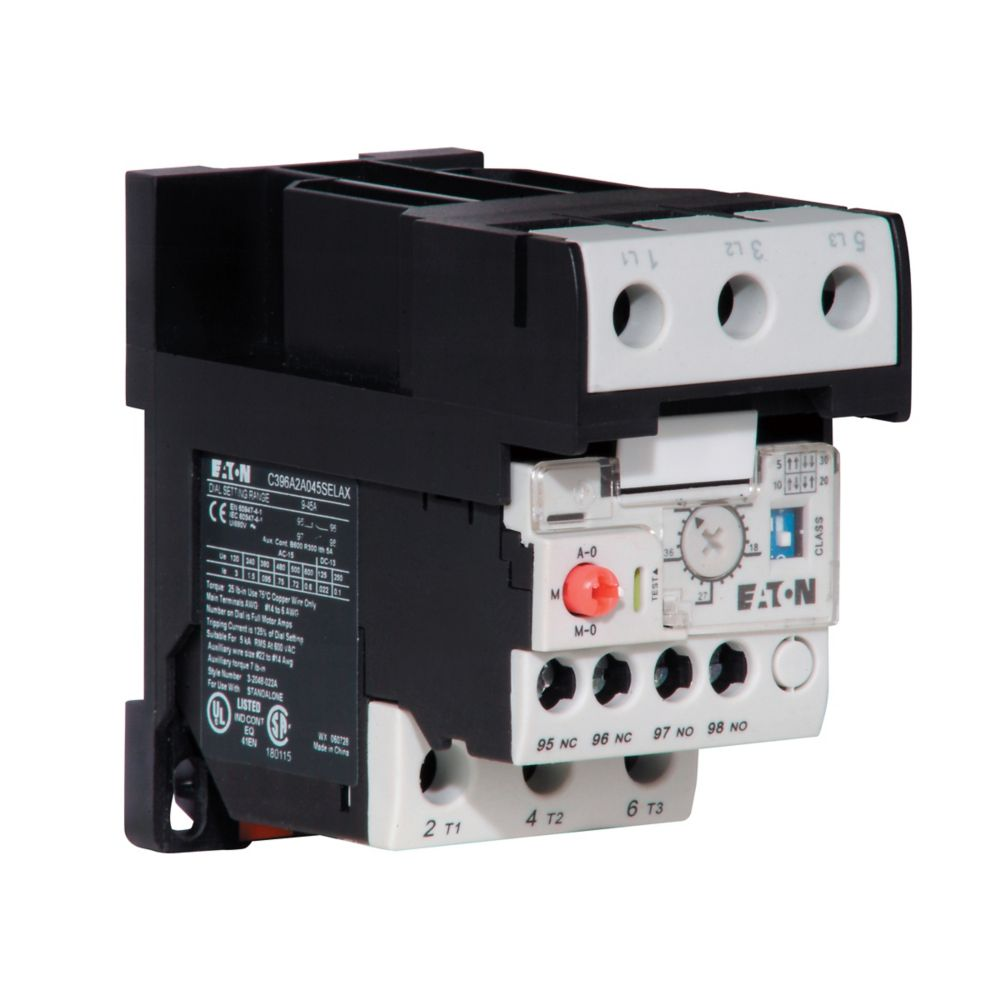
\includegraphics[width=\textwidth]{Imagenes/relevador}
		\caption{Relé de protección térmica Eaton \cite{Eaton2}.}
		\label{fig:rele}
	\end{subfigure}
\caption{Elementos de control y protección de motores.}
\end{figure}


Un relé de sobrecarga es un dispositivo de protección utilizado para evitar el sobrecalentamiento del motor eléctrico; la Figura \ref{fig:rele} muestra un relé de sobrecarga electrónico. Estos se clasifican en dos grandes tipos: Los térmicos y los electrónicos. Los relés térmicos detectan el aumento de temperatura del motor y, si la temperatura excede un cierto umbral, desconectan el motor para evitar daños. Los relés térmicos funcionan mediante el uso de elementos de medición de temperatura, como fusibles de alección eutéctica o bimetálicos, que desconectan los contactos del relé en caso de sobrecalentamiento.

Por otra parte los relés electrónicos posee una electrónica auto-alimentada con termistores que posee las siguientes características: poseen disparo ajustables para una protección óptima en diferentes condiciones de arranque, detectan  perdida de fase y desbalance, poseen liberación automática/manual para un rápido reinicio del proceso para una mayor disponibilidad, poseen una sensibilidad monofásica ajustable para cargas simétricas y asimétricas, detección integrada de la corriente de defecto a tierra en algunos casos y no requieren compensación térmica como los elementos térmicos. 


En conjunto, el contactor y el relé térmico se le llama arrancador electromagnético y se utilizan comúnmente en el control eléctrico de motores para proporcionar una interrupción segura y eficiente. Cuando se utiliza un contactor y un relé térmico en combinación, el contactor controla la conexión y desconexión del motor, mientras que el relé térmico proporciona protección contra  el sobrecalentamiento del motor.

\subsection{Curvas de disparo}

Las curvas clase 10, 20 y 30 son curvas de tiempo de disparo utilizadas en los elementos térmicos del relés según la norma NEMA (National Electrical Manufacturers Association) para la protección de motores eléctricos, ver Figura \ref{fig:curvasclass}.

Cada curva indica el tiempo tiempo de apertura del circuito  en función de la corriente de sobrecarga. La norma NEMA especifica los valores de corriente para cada curva son:

Curva clase 10: Esta curva se dispara en un tiempo de 10 segundos a una corriente de sobrecarga igual a 600\% de la corriente nominal del motor.

Curva clase 20: Esta curva se dispara en un tiempo de 20 segundos a una corriente de sobrecarga igual a 600\% de la corriente nominal del motor.

Curva clase 30: Esta curva se dispara en un tiempo de 30 segundos a una corriente de sobrecarga igual a 600\% de la corriente nominal del motor.

Es importante tener en cuenta que estas curvas de tiempo de disparo son solo una guía para la selección de los elementos térmicos, y la selección final dependerá de las características específicas del motor y la aplicación. Adicionalmente es importante que exista un correcta coordinación con el dispositivo de protección contra corto-circuito (SCPD) o breaker. La Figura \ref{fig:cordinacion} muestra el comportamiento de la corriente de un motor, la curva de protección térmica, la curva del SCPF y la curva que define la zona en que el motor se daña.

\begin{figure}
	\centering
	\begin{subfigure}[b]{0.48\textwidth}
		\centering
	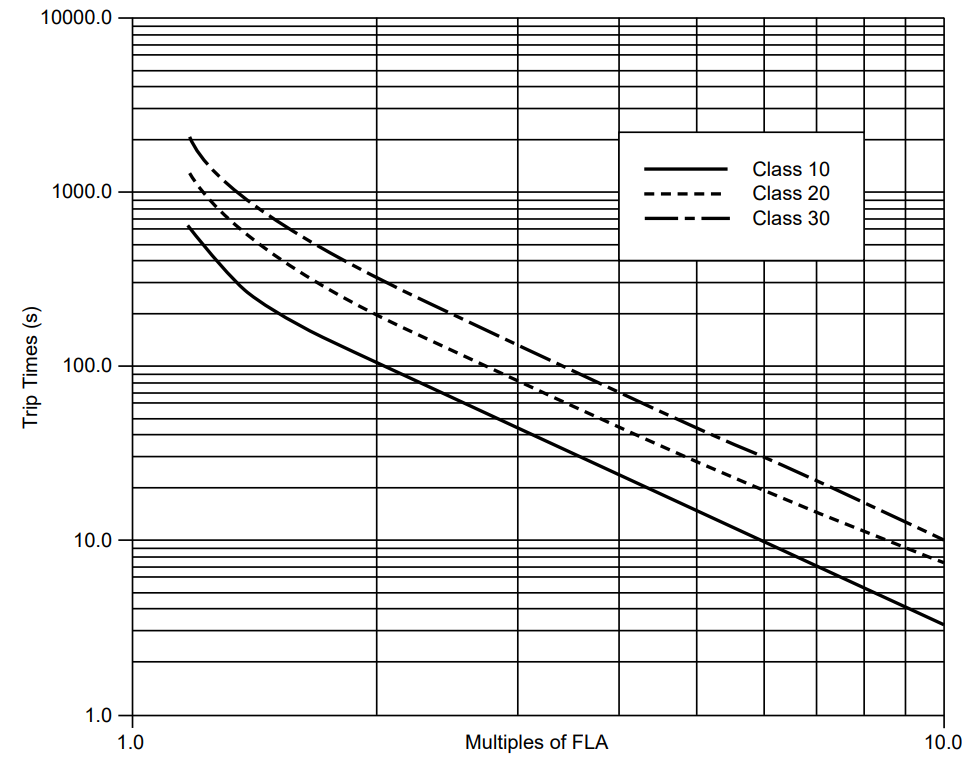
\includegraphics[width=\textwidth]{Imagenes/CurvasClass}
	\caption{Curvas NEMA Clase 10 , 20 , 30.}
	\label{fig:curvasclass}
	\end{subfigure}
	\hfill
	\begin{subfigure}[b]{0.5\textwidth}
		\centering
		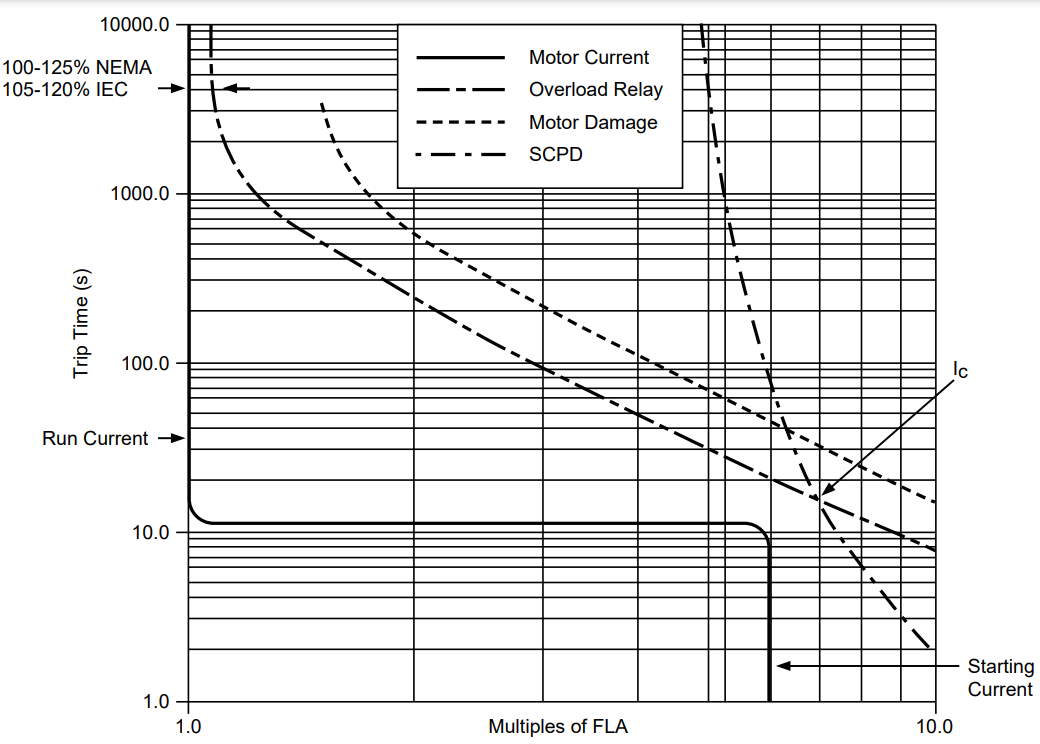
\includegraphics[width=\textwidth]{Imagenes/Cordinación}
		\caption{Coordinacion de curvas y zona de daño del motor.}
		\label{fig:cordinacion}
	\end{subfigure}
	\caption{Curvas de protección térmica \cite{Scheneider}.}
\end{figure}


\subsection{Selección de componentes}

Usualmente cada fabricante propone su procedimiento de selección para contactores o relevadores, sin embargo los procedimientos tienen criterios comunes. Usualmente los contactores se seleccionan por: potencial del motor, voltaje de línea, voltage de la bobina, frecuencia de la red, vida útil (o cantidad de operaciones mínima requerida) y tipo de protección ambiental que se requiera, esto último se refiere al tipo de gabinete donde se monta el contactor. 
Por otra parte, los relevadores se seleccionan según la corriente nominal, la aplicación determina el tiempo de disparo de la curva, el tamaño del contactor al que debe ser acoplado y la compensación ambiental sólo en relevadores térmicos.  

  
\section{Metodología}

Este laboratorio tiene una duración de 4 lecciones, repartidas en dos semanas. Los estudiantes deben mostrar durante las clases programadas las tres actividades propuestas. Deben recabar fotografías y resultados de los equipos de medición para elaborar las evidencias. Las evidencias se subirán al TecDigital la semana siguiente finalizadas las actividades.

\section{Práctica en Clase}

\subsection{Actividad 1}

 Se desea seleccionar un arrancador térmico para dos motores que mueve una bomba de agua. El primer motor es de 100 hp, trifásico (3$\varnothing$), voltaje de línea 480 voltios, voltaje de control de 120 voltios. No se requiere gabinete. El segundo motor es de 50 hp, 3$\varnothing$, 240V, 60Hz, voltaje control 120 V, ambos a plena carga con factor de potencia 0.95 en atraso. Asuma eficiencias del motor de 86\%. Por ejemplo las bombas se usan en promedio 3 veces al día todos los días y se requiere que los contactores duren al menos 20 años. 
 
\subsubsection{Conteste las preguntas}

¿Cual sería para ambos aplicaciones el modelo de arrancador con reveladores electrónicos con falla a tierra para la marca EATON según el catalogo \href{https://www.eaton.com/content/dam/eaton/products/industrialcontrols-drives-automation-sensors/nema-contactors-and-starters-v5-t2-ca08100006e.pdf}{\textit{NEMA Contactors and Starters}}, serie Freedom?. ¿Puede explicar porque se usa el mismo contactor para ambos casos?


\subsection{Actividad 2}
  Los ingenieros Electricistas, electromecánicos y de Mantenimiento pueden diseñar sus circuitos de control eléctrico, sin embargo cada fabricante posee libros de diagramas estandarizados como el que brinda  Schneider con su documento \href{https://download.schneider-electric.com/files?p_enDocType=Catalog&p_File_Name=0140CT9201.pdf&p_Doc_Ref=0140CT9201&_ga=2.160182845.1491407618.1677858387-1733391740.1677858387}{\textit{Wiring Diagram Book}}\cite{Scheneider2}.
 
 Estudie toda la simbología NEMA, Tabla 1 y Tabla 2 de la referencia \cite{Scheneider2} y asocie los con el elementos físicos y su funcionamiento.
 Deduzca la ecuación lógica del circuito eléctrico de control, para esto use un mapa de Karnaugh o la ecuacion caracteristica del cerrojo S-R prioridad al reset.
 Realice el alambrado del circuito de control y luego del circuito de potencia del arranque sencillo de un motor trifásico de 1/2 hp.
 
 
\subsubsection{Conteste las preguntas:}

¿Es el circuito alambrado control a dos o tres hilos? Explique. ¿El circuito de control funcionó según la tabla de verdad?, Que pasa si se pierde una fase, como se comporta el circuito?. Que diferencia existe entre un arrancador automático y uno manual en el caso que exista un corte de flujo eléctrico? Explique.
 Hasta ahora los circuitos fueron representados según la norma NEMA, muestre el circuito de control y potencia según la simbología de la norma IEC.

\subsection{Actividad 3}

Deduzca el circuito de control de un arranque-pare-reversive. Realice el alambrado del circuito de control y luego del circuito de potencia del circuito para un trifásico de 1/2 hp.

\subsubsection{Conteste las preguntas:} 

 ¿El circuito de control funcionó según la tabla de verdad?, ¿Que pasa si se presionan los botones pulsadores de arranque hacia la derecha y arranque hacia la izquierda al mismo tiempo? Explique usando el concepto de enclavamiento. 
 Muestre el circuito de control y potencia según la simbología de la norma IEC.



